% begin module horizontal-line-test
\begin{frame}
Question: How can we tell from the graph of a function whether it is one-to-one or not?

Answer: Use the horizontal line test.

\begin{proof}[The Horizontal Line Test]
A function is one-to-one if and only if no horizontal line intersects it more than once.
\end{proof}

\begin{tabular}{cc}
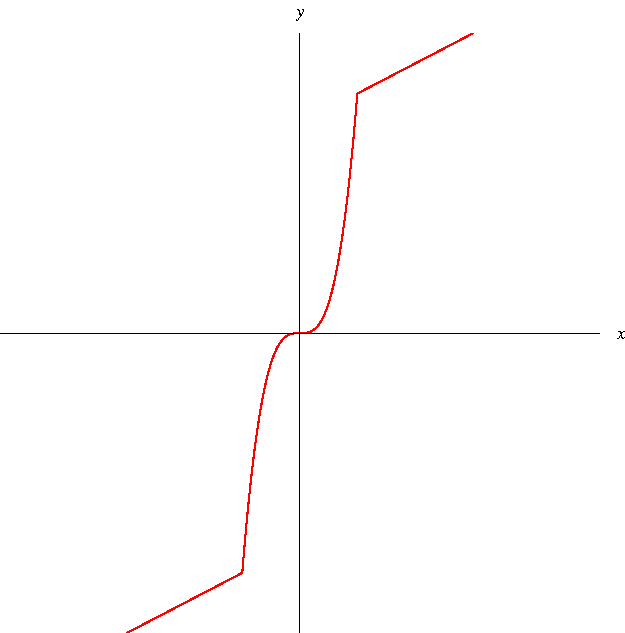
\includegraphics[height=4cm]{inverse-functions/pictures/07-01-onetoone.pdf} &%
\only<handout:0| -2>{%
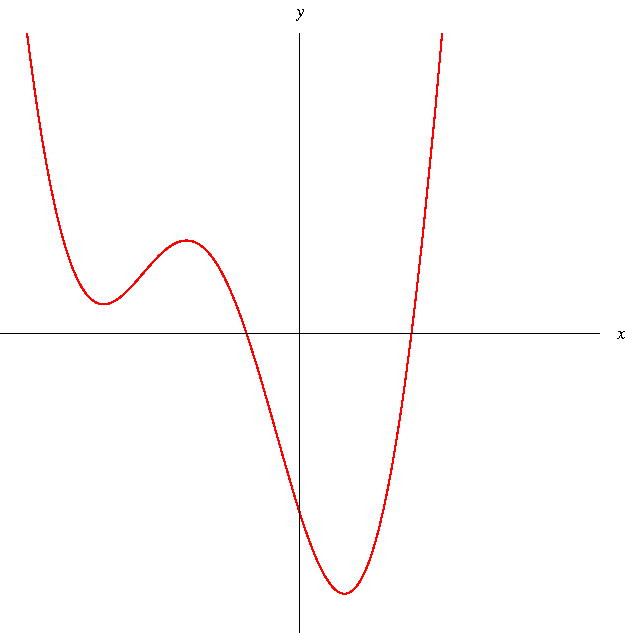
\includegraphics[height=4cm]{inverse-functions/pictures/07-01-notonetoonea.pdf}%
}%
\only<handout:1| 3->{%
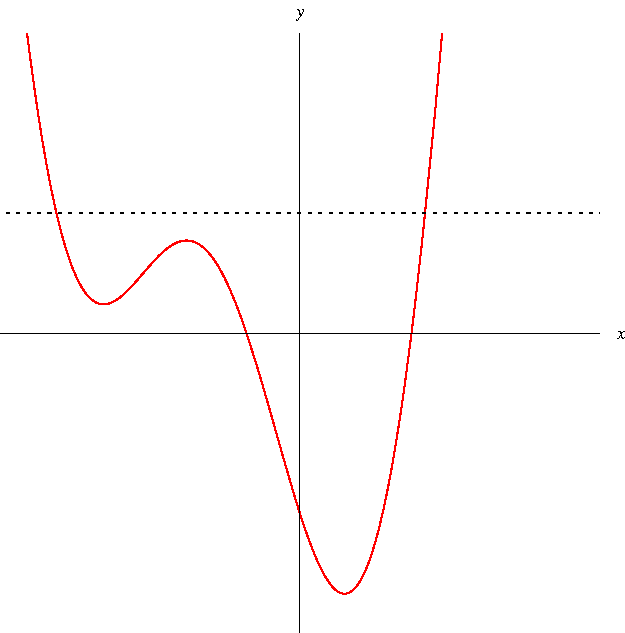
\includegraphics[height=4cm]{inverse-functions/pictures/07-01-notonetooneb.pdf}%
}\\
\uncover<2->{\alert<handout:0| 2>{One-to-one}} &
\uncover<3->{\alert<handout:0| 3>{Not one-to-one}}
\end{tabular}
\end{frame}
% end module horizontal-line-test
